This section describes the overall proposal architecture for robo-actors. This description is divided into two views. 

The first view show the structural composition of an roboactor and describes generally which responsibilities its internal structures have(responsibilities of all the blue boxes in the image).

The architecture could be seen in the Figure~\ref{fig:generalArchitecture}. 
\todo[inline]{I made some changes in the image of the architecture}
 \todo[inline]{In the caption of the architecture should be finished the explanation of the arrows, which is not so clear if there is additional meaning}
\begin{figure}
	\centering
	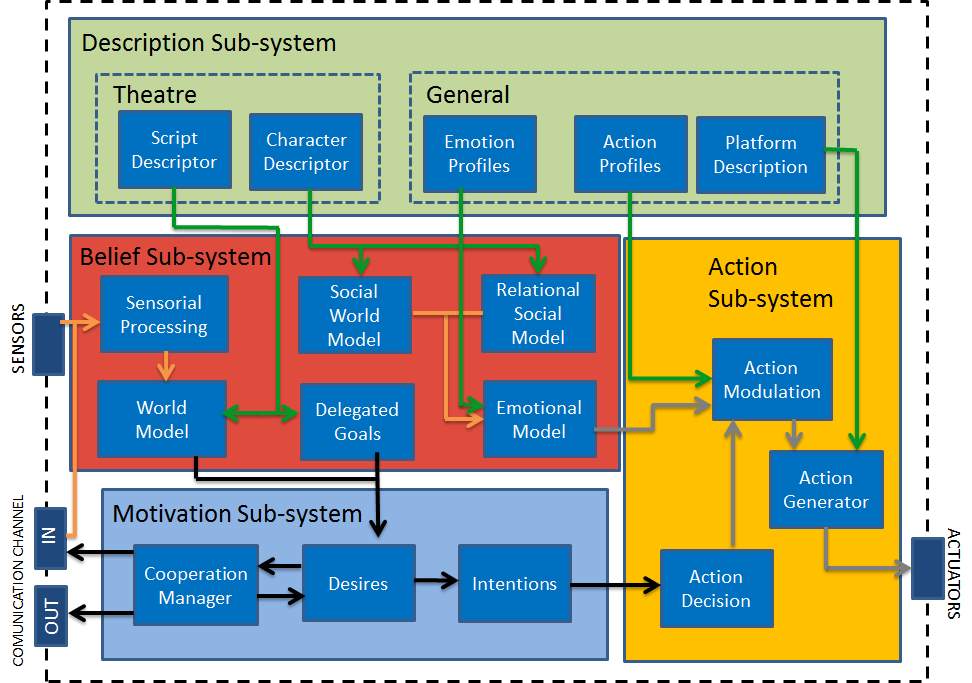
\includegraphics[width=0.5\textwidth]{Images/GeneralArchitecture.png} 
	\caption{General architecture . The green arrows show the information that comes from the description sub-system. The orange arrows are information that is share in the belief sub-system.}
	\label{fig:generalArchitecture}
\end{figure}

The second view is the behavioral structure in a general way. Also, It can be divided in two parts:

First, describes the internal behavior of beliefs in a robo-actor in which is important highlight the emotional and knowledge representation in relationship with the theatre context.

The second part is dedicated to the cooperation mechanisms and deliberation process through which the robots are able to coordinate and act.